\section{Data space estimators}

\subsection{Deriving the data space estimators}

We start by defining the model error as the expectation across models of the
$\chi^2$ between the model predictions and some data central values
$\levone^\prime$, normalised by the number of data points
\begin{equation}
    \label{eq:chi2kerep}
    \eout = \frac{1}{\ndata} \erep{
        \left( \model\left(u_*^{\repind}\right) - \levone^\prime \right)^T
        \invcovprime
        \left( \model\left(u_*^{\repind}\right) - \levone^\prime \right)
    }\, ,
\end{equation}
where we purposely denoted the data which the model error is evaluated on as
$\levone^\prime$, as opposed to the data which is used to determine the model
parameters $\levone$. We could of course set $\levone^\prime = \levone$ and
evaluate the model performance on the fitted data however, as is common in
machine learning literature, we intend to use a separate set of test data.
Ideally we would choose $\levone^\prime$ such that $p(\levone^\prime, \levone) =
p(\levone^\prime)p(\levone)$, in other words the training and test set are
statistically independent. To make things unambiguous we will denote the model
error, when evaluated on the ideal case of $\levone^\prime$, as $\eout$. In the
context of a closure test, $\eout$ is a stochastic quantity which depends both
on the training data, through the model predictions and the test data.

We can gain some insight by performing a decomposition of this expression, a
similar exercise is performed for the likelihood function associated with
least-squares regression in \cite{mlforphysics}. Least-squares regression is a
special case of maximum likelihood estimation, where the uncertainty on each
data point is equal in magnitude and uncorrelated. Here we review the
decomposition in the more general framework of data whose uncertainty is
multigaussian. While the two computations are simply related by a change of
basis in the space of data, it is useful to have explicit expressions with the
full covariance matrix, which are closely related to the ingredients that are
usually entering a fit. Starting with Eq.~\ref{eq:chi2kerep} (evaluated on the
ideal test data), we can expand the square
\begin{equation}
    \begin{split}
    \label{eq:EoutDecomposition}
        &\eout = \frac{1}{\ndata} \left( \erep{
            \left( \model\left(u_*^{\repind}\right) - f^\prime \right)^T
            \invcovprime
            \left( \model\left(u_*^{\repind}\right) - f^\prime \right)
        } + \right. \\
        &+ %\erep{
            \left( f^\prime - \levone^\prime \right)^T
            \invcovprime
            \left( f^\prime - \levone^\prime \right)
        %}
        + \\
        &\left. + 2 \erep{
            \left( \model\left(u_*^{\repind}\right) - f^\prime \right)^T
            \invcovprime
            \left(f^\prime - \levone^\prime \right)
        }\right) \, .
    \end{split}
\end{equation}
Let us discuss these three contributions in turn. The second term is the
contribution associated with evaluating the model error on noisey data, we will
refer to this term as {\em noise}, while the final term is a cross term which we
will deal with later. We can decompose the first term further,
% TODO: add the same thing but for fully in sample data to an appendix.
\begin{equation}
    \begin{split}
        &\erep{
            \left( \model\left(u_*^{\repind}\right) - f^\prime \right)^T
            \invcovprime
            \left( \model\left(u_*^{\repind}\right) - f^\prime \right)
        } = \\
        &= \erep{
            \left( \model\left(u_*^{\repind}\right) - 
            \erep{\model\left(u_*^{\repind}\right)} \right)^T
            \invcovprime
            \left( \model\left(u_*^{\repind}\right) - 
            \erep{\model\left(u_*^{\repind}\right)} \right)
        } + \\
        &+ \left( \erep{\model\left(u_*^{\repind}\right)} - f^\prime \right)^T
        \invcovprime
        \left( \erep{\model\left(u_*^{\repind}\right)} - f^\prime \right)\, ,
    \end{split}
\end{equation}
where we have used the fact that the second term is constant across replicas and
the cross term that arises in this decomposition is zero when the expectation
value across replicas is taken. The first term in this expression we call the
variance and the second term is the bias.

As previously mentioned $\eout$ should be considered a stochastic estimator, in
theory we could take the expectation value across training data $\levone$ and
test data $\levone^{\prime}$, the latter of which cancels the cross term in
Eq.~\ref{eq:EoutDecomposition}. The final result of that would be
\begin{equation}\label{eq:ExpectedBiasVariance}
    \mathbf{E}_{\levone, \levone^\prime}[\eout] =
    \mathbf{E}_{\levone}[{\rm bias}] + 
    \mathbf{E}_{\levone}[{\rm variance}] + 1\, .
\end{equation}
We are not interested in the observational noise term, since it is
independent of the model. The two estimators of interest are independent of
the test data, and therefore we only need to take the expectation value on
the training data.
\paragraph{Multiple closure fits}
In practical terms, taking the expectation value across the training data can
be achieved by running multiple closure fits, each with a different
observational noise vector $\shift$, and taking the average i.e.
\begin{equation}
    \mathbf{E}_{\levone}[ \cdot ] = \frac{1}{\nfits} \sum_{j=1}^{\nfits} \cdot.
\end{equation}
Clearly this is resource intensive, and requires us to perform many fits. In
NNPDF3.0 \cite{nnpdf30}, single replica proxy fits were used to perform a study
of the uncertainties. Here we have expanded the estimators used in the closure
fits and also will be using multiple full replica fits to calculate various
expectation values - made possible by our next generation fitting code.

\subsection{Geometric Interpretation}

It is possible to interpret the relevant data space estimators geometrically, by
considering a coordinate system where each basis vector corresponds to an
eigenvector of the experimental covariance matrix normalised by the square root
of the corresponding eigenvalue. The origin of the coordinate system is the true
value of the observable. The model predictions are then a set of points, where
the mean squared radius of those points is what we call the variance. The bias
is the l2-norm of the vector between the origin and the mean of the model
predictions. An example of this is given in Fig.~\ref{fig:diagram2destimators},
where for simplicity we have considered a system with just two data points, \ie\
a two-dimensional data space, with a diagonal covariance.
%
\begin{figure}
    \centering
    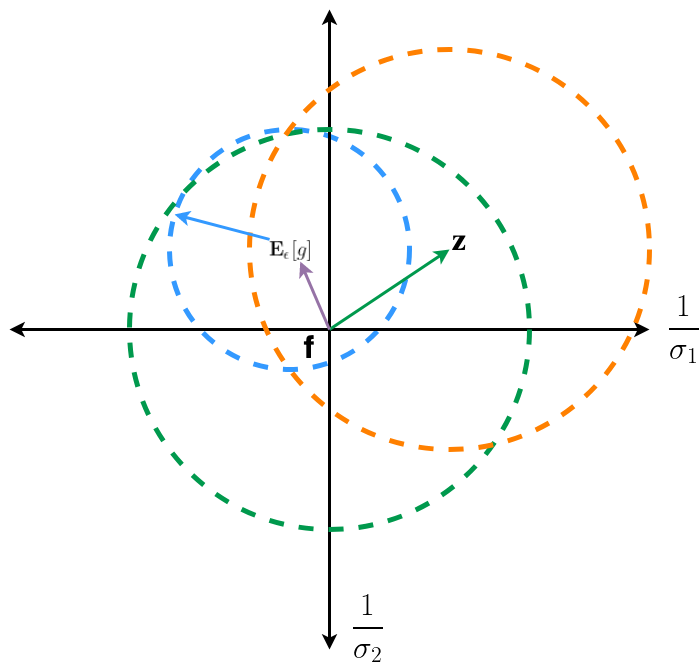
\includegraphics[width=0.8\textwidth]{diagonal_basis_2d_estimators_diagram.png}
    \caption{Example of geometric interpretation of closure test estimators.
    The origin
    is the true observable values for each data point. The level one data (or
    experimental central values) are
    shifted away from this by $\shift$. In this example the covariance matrix
    is diagonal, so the eigenvectors correspond to the two data points, the
    square root of the eigenvalues are simply the standard deviation of those
    points. This is without loss of generality because any multivariate distribution
    can be rotated into a basis which diagonalises the covariance matrix.
    The 1-sigma observational noise confidence interval
    is a unit circle centered on the origin. Some closure
    estimators can be understood as l2-norms of the vectors connecting points,
    i.e the bias is the l2-norm of the vector from the origin to the central
    value of the predictions.}
    \label{fig:diagram2destimators}
\end{figure}
%
\subsection{Faithful uncertainties in data space}

The two closure estimators of interest, bias and variance, can be used to
understand faithful uncertainties in a practical sense. If we return to
Eq.~\ref{eq:ExpectedBiasVariance} we can examine both estimators in a bit more
detail.

\paragraph{Variance}

The {\em variance} in the above decomposition refers to the variance of the
model predictions in units of the covariance
\begin{equation}
    \label{eq:VarDef}
    \var = \frac{1}{\ndata}
    \erep{
            \left( \model\left(u_*^{\repind}\right) - 
            \erep{\model\left(u_*^{\repind}\right)} \right)^T
            \invcovprime
            \left( \model\left(u_*^{\repind}\right) - 
            \erep{\model\left(u_*^{\repind}\right)} \right)
        }\, ,
\end{equation}
which can be interpreted as the model uncertainty in the space of the test data.
It is instructive to rephrase Eq.~\ref{eq:VarDef} as
\begin{equation}
    \label{eq:VarDefalternative}
    \var = \frac{1}{\ndata} {\rm Tr} \left[ \covrep \invcovprime \right],
\end{equation}
where 
\begin{equation}
    \label{eq:CovRep}
    \covrep = 
    \erep{
            \left( \model\left(u_*^{\repind}\right) - 
            \erep{\model\left(u_*^{\repind}\right)} \right)
            \left( \model\left(u_*^{\repind}\right) - 
            \erep{\model\left(u_*^{\repind}\right)} \right)^T
        }
\end{equation}
is the covariance matrix of the predictions from the PDF replicas. Going to a
basis where $\invcovprime$ is diagonal,
\begin{equation}
    \label{eq:InvCovPrimeDiag}
    \left(\invcovprime \right)_{ij} = \frac{1}{\left(\sigma'_i\right)^2} 
    \delta_{ij}\, ,
\end{equation}
we can rewrite Eq.~\ref{eq:VarDefalternative} as 
\begin{equation}
    \label{eq:VarianceInterpretation}
    \var = \frac{1}{\ndata}\, \sum_i \frac{\covrep_{ii}}{\left(\sigma'_i\right)^2}\, .
\end{equation}
The numerator in the right-hand side of the equation above is the variance of
the theoretical prediction obtained from the fitted replicas, while the
denominator is the experimental variance. Hence the right-hand side of the
equation is the average reduction in the variance of the observables between the
prior distribution, dictated by the experimental covariance, and the posterior
distribution. The average is computed over the space of test data, \ie\ data points that are not seen by the fit. 

\paragraph{Bias}

Similarly, the {\em bias}\ is defined as the difference between the expectation
value of the model predictions and the true observable values in units of the
covariance, \ie 
\begin{equation}
    \label{eq:BiasDef}
    \bias = \frac{1}{\ndata}
    \left( \erep{\model(u_*^{\repind})} - f^\prime \right)^T
        \invcovprime
    \left( \erep{\model(u_*^{\repind})} - f^\prime \right)\, .
\end{equation}
The smaller the bias, the closer the central value of the predictions is to the
underlying law. In Eq.~\ref{eq:ExpectedBiasVariance}, the expectation value is
taken across the prior distribution of the training data, which yields
\begin{equation}
    \mathbf{E}_{\levone}[{\rm bias}] = \frac{1}{\ndata}
    {\rm Tr} \left[ \covcent \invcovprime{} \right]\, ,
\end{equation}
where we have introduced $\covcent$ as the covariance of the expectation value
of the model predictions,
\begin{equation}
    \label{eq:CovCentDef}
    \covcent = 
    \mathbf{E}_{\levone}\left[
        \left( \erep{\model(u_*^{\repind})} - f^\prime \right)
        \left( \erep{\model(u_*^{\repind})} - f^\prime \right)^T   
    \right]\, .
\end{equation}
The point is that the bias on the test data is a stochastic variable which
depends on the central value of the training data through $u_*^{\repind}$. The
matrix $\covcent$ describes the fluctuations of the central value of the model
prediction around the true observable values as we scan different realisations
of the training data. 

It is important to stress the difference between variance and bias. In the case
of the variance, we are looking at the fluctuations of the replicas around their
central value for fixed $\vv{\levone}$. This is what is done in a fit to real
data, where we have one instance of $\vv{\levone}$, provided by the experiments.
In the case of the bias we consider the flucutations of the central value over
replicas around the true theoretical prediction as the values of $\vv{\levone}$
fluctuate around $\vv{\law}$. This latter procedure is only possible in a
closure test, where the underlying true theoretical prediction is known. The
bias as defined here yields an estimate of the fluctuations of the MAP estimator
if we could do multiple independent experiments. 

% If we take the expectation across training data, then we get a distribution of
% expectation values of model predictions. The true observable values are
% static, and not drawn from a distribution, however the difference between the
% expected value of our model and the truth is probabilistic and in practical
% terms the uncertainties of our model predictions should be consistent with the
% observed distance from the truth.

\paragraph{Bias-variance ratio}

Finally, the {\em bias-variance ratio} is defined as
\begin{equation}
    \label{eq:RatioDef}
    \biasvarratio \equiv \sqrt{\frac{\eshift{\bias}}{\eshift{\var}}}\, ,
\end{equation}
where we have taken the square root, since bias and variance are both mean
squared quantities. The value of $\biasvarratio$ yields a measurement of how
much uncertainties are over or under estimated. If the uncertainties are
completely faithful, then $\biasvarratio = 1$. We note that the relationship
does not work both ways and $\biasvarratio = 1$ does not necessarily guarantee
that the uncertainty is faithful. We also note that $\biasvarratio$ is not
completely general: it is not a measure defined in model space and depends on
the choice of test data. Therefore it only gives 'local' information on the
model uncertainties. If the distribution of the expectation value of model
predictions is gaussian centered on the true observable values, with covariance
$\covcent$ and the distribution of the model replicas is also gaussian, with
covariance $\covrep$ then model uncertainties are faithful if
\begin{equation}\label{eq:IdealRatioDef}
    \covcent {\covrep}^{-1} = 1.
\end{equation}
The difficulty with calculating Eq.~\ref{eq:IdealRatioDef} comes from the fact
that $\covrep$ is likely to have large correlations which would lead it to be
singular or ill-conditioned. As a result, any error estimating $\covrep$ from
finite number of replicas could lead to unstable results. $\biasvarratio$
overcomes this instability by taking the ratio of the average across test data
of these matrices, in units of the experimental covariance matrix. There may
still be large relative errors for smaller eigenvalues of $\covrep$, but these
should not lead to instabilities in $\biasvarratio$ unless they correspond to
directions with very low experimental uncertainty. As an extra precaution, we
shall estimate an uncertainty on $\biasvarratio$ by performing a bootstrap
sample on fits and replicas.
% TODO: summaries that bias and variance are performance estimators but must
% remain balanced?

\paragraph{Quantile statistics}

A closure test estimator which was previously defined in \cite{nnpdf30}, in
the space of PDFs was
$\xi_{1\sigma}$. We define here an analogous estimator in data space
\begin{equation}
    \label{eq:XiDataDef}
    \xi_{1\sigma} = 
        \frac{1}{\ndata} \sum_{i}^{\ndata} 
        \frac{1}{\nfits} \sum_{l}^{\nfits}
            I_{[-\sigma_i^{(l)}, \sigma_i^{(l)}]}
            \left( \erep{\model_i}^{(l)} - \law_i \right),
\end{equation}
where $\sigma^{(l)}$ is the standard deviation of the theory predictions
estimated from the replicas of fit $l$. $\xi_{1\sigma}$ aims to measure the same
thing as $\frac{\eshift{\bias}}{\eshift{\var}}$: whether the distribution of
replicas for a given fit matches the distribution of the central predictions
around the underlying predictions.
%TODO: discussion of comparison

\subsection{Discussion of xi, some of which should go in subsection above}

where $\sigma^{(l)}$ is the standard deviation of the theory predictions
estimated from the replicas of fit $l$. $\xi_{1\sigma}$ aims to measure the same
thing as $\frac{\eshift{\bias}}{\eshift{\var}}$: whether the distribution of
replicas for a given fit matches the distribution of the central predictions
around the underlying predictions. It is useful to define $\xi_{1\sigma}^{i}$ as
the value of $\xi_{1\sigma}$ for an individual data point such that
\begin{equation}
    \label{eq:XiDataIDel}
    \xi_{1\sigma} = \frac{1}{\ndata} \sum_i \xi_{1\sigma}^{i}.
\end{equation}
If we assume that the replica distribution is constant across fits then our
definition $\xi_{1\sigma}^{i}$ is just a discretised expectation value of the
indicator function. In the case that we have infinite fits, then
\begin{equation}
    \label{eq:XiIExpecVel}
    \xi_{1\sigma}^{i} = 
    \int_{-\infty}^{\infty} I_{[-\sigma_i, \sigma_i]}\, 
    p(\erep{\model_i} - \law_i)\, 
    {\rm d}(\erep{\model_i} - \law_i).
\end{equation}
If we then assume that $p(\erep{\model_i} - \law_i)$ is a gaussian centered on
zero with a standard deviation which we will denote as $\modelstd_i$ then the
integral simplifies to
\begin{equation}
    \label{eq:expectedxi}
    \xi_{1\sigma}^{i} = 
    \erf \left( \frac{\sigma_i}{\modelstd_i \sqrt{2}}\right),
\end{equation}
which is the standard result of integrating a gaussian over some finite
symmetric interval. Clearly if the distribution of central predictions about the
underlying law matches the distribution of the replica predicitons around the
central predictions then the expected value of $\xi_{1\sigma}^{i}$ is 0.68. This
is consistent with the assumptions we made, \viz\ it is  the quantile statistics
of a gaussian distribution.

One can also look at the variance of the indicator function across fits to get
an idea of the fluctuation of $\xi_{1\sigma}^{i}$, which we will denote as
$\Delta[\xi_{1\sigma}^{i}]$
\begin{equation}
    \label{eq:XiIVar}
    \begin{split}
        \Delta[\xi_{1\sigma}^{i}] 
        =& \int_{-\infty}^{\infty} I_{[-\sigma_i, \sigma_i]}^2\, 
            p(\erep{\model_i} - \law_i)\,
            {\rm d}(\erep{\model_i} - \law_i) - \\
        &- \left( \int_{-\infty}^{\infty} I_{[-\sigma_i, \sigma_i]}\,
            p(\erep{\model_i} - \law_i)\,
            {\rm d}(\erep{\model_i} - \law_i) \right)^2,
    \end{split}
\end{equation}
which can be simplified to
\begin{equation}
    \label{eq:XiIVarSimplified}
    \Delta[\xi_{1\sigma}^{i}] =
    \erf \left( \frac{\sigma_i}{\modelstd_i \sqrt{2}}\right) -
    \erf \left( \frac{\sigma_i}{\modelstd_i \sqrt{2}}\right)^2.
\end{equation}
Even in the ideal case that the distributions are the same, we see that the
$\Delta[\xi_{1\sigma}^{i}] = 0.22$, which is a large spread considering
$\xi_{1\sigma}^{i}$ is bounded between 0 and 1.

When taking the mean across datapoints to obtain $\xi_{1\sigma}$ we note that
getting 0.68 relies on each sampled $\xi_{1\sigma}^{i}$ being statistically
independent. This clearly will not be the case because there can be a big
correlation between datapoints within the same dataset. We can calculate
$\xi_{1\sigma}$ in different basis and note that unlike $\chi^2$ and quantities
of the form $v^T M v$, $\xi_{1\sigma}$ is not basis independent. There is a
choice of basis, however it will be useful to compare the value $\xi_{1\sigma}$
and $\frac{\eshift{\bias}}{\eshift{\var}}$. Therefore, a natural basis to
calculate $\xi_{1\sigma}$ is the basis which diagonalises the experimental
covariance matrix because bias and variance are both calculated in units of the
experimental
% Should I mention this without having tried it?
covariance. As previously discussed, this makes sense in light of using the PDFs
to make data-theory comparisons.
